\section{Sound System}
The sound system can be seen as an thread except it is not awaken by the operating system scheduler but rather by the Interrupt system. It relies heavily on 
\par
PIT chips runs at 1.193182 MHz. That looks like an odd number which is once again due to history. Back in the 1980, when the first IBM PC 5150 was being designed, the common oscillator used in television circuitry was running at 14.31818 MHz. In order to reduce part cost, engineers built the PC timer around it dividing the frequency by 3 for the CPU (that is why the Intel ran at 4.7), dividing by 4 to 3.57Mhz for the CGA video card. By logically ANDing these signals together a frequency equivalent to the base frequency divided by 12 was created. This frequency is 1.1931816666 MHz. By 1991 the oscillator were much cheaper and it could have been anything....but backyward compatibility once again forbid it.\\
\par
At the heart of the PC, is the oscillator programmed via Programmable Interval Timer (PIT).\\



\subsection{Architecture}




\subsection{Music}
IMF format. 0 sound effects, 8 channels for music. IMF files store the actual bytes sent to the AdLib's OPL2 chip, which uses FM synthesis to produce audio output.

How to program the AdLib: quote trixter

The Adlib (and the FM portion of the Sound Blaster, as it's a clone of the Adlib) is controlled by sending a series of instructions to a certain port (388h). When the Adlib was first conceived in 1986, it was tested on IBM PCs and ATs, none of which exceeded a speed of 6 MHz. They wrote their specification based on this, writing that while the Adlib required a certain amount of "wait time" between commands, it was okay to send them as fast as possible because no PC was faster than the minimum wait time. They later found out that a 386 was fast enough to send commands faster than the Adlib was expecting them, and they changed their specification to mention a minimum 35ms wait time between commands.

Unfortunately, some games (Sky Shark, Budokan, and Windwalker, amongst others) had already been published using the older specification. Running these on today's modern PCs produces garbled sound because the FM chip on your sound card is being pushed beyond it's original specification.

I talked to Jason Linhart, the founder and lead programmer of MicroMagic, in 1997 about this very phenominon in Windwalker:

"The original AdLib manual (before they shipped) did not call for ANY delays. The original IBM PC (4.77 Mhz) couldn't get ahead of the card. By the time it shipped they were telling use to do one IN instruction, and every time a new faster processor came out they added some delay to their recomendation. The old 8088 machines would not have worked with the 35 IN instructions now required, it would have slowed the machine down so much nothing else could get done."


\subsection{Sound effects}
\par
\begin{figure}[H]
\centering
 \fullimage{audio/audio_settings.png}
 \end{figure}
\par

\subsubsection{PCM}


\subsubsection{Solving the PC Speaker problem: PWM}
Pulse Width Modulation, or PWM, is a technique for getting analog results with digital means.




\par
 \begin{fancyquotes}
  The PC speaker is normally meant to reproduce a square wave via only 2 levels of output (the speaker is driven by only two voltage levels, typically 0 V and 5 V). However, by carefully timing a short pulse (i.e. going from one output level to the other and then back to the first), and by relying on the speaker's physical filtering properties (limited frequency response, self-inductance, etc.), the end result corresponds to intermediate sound levels. This effectively allows the speaker to function as a crude 6 bit DAC,[5] thereby enabling approximate playback of PCM audio. This technique is called pulse-width modulation (PWM).
 \end{fancyquotes}
\par
  It gave surprisingly good results such as in Monkey Island music.\footnote{https://www.youtube.com/watch?v=a324ykKV-7Y}

  \par
The programming trick in the PC was to set the timer that drive PC speaker to one-shot mode, and set PC interrupt rate to needed output sample rate. So at every input one sound sample value was read, converted to timer control value, programmed to timer (starting the pulse). This trick allowed around 6 bits sample resolution / dynamics (or even slightly more with some tricks). When the sample rate was high enough, you can’t hear the high frequency noise on the signal.\\
TODO: Drawing of PWM
\par
Mode 1 - Hardware Re-triggerable One-shot\\
Mode 2 - Rate Generator\\
Mode 3 - Square Wave Generator\\
Mode 4 - Software Triggered Strobe\\
Mode 5 - Hardware Triggered Strobe\\
\par
\begin{figure}[H]
\centering
 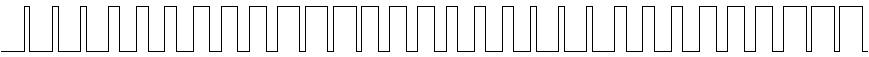
\includegraphics[width=\textwidth]{imgs/drawings/pwm/sinuois.png}
 \end{figure}
\par

\par
\begin{figure}[H]
\centering
 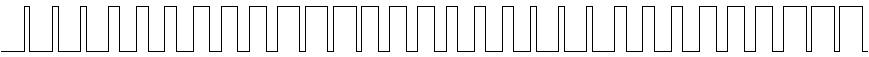
\includegraphics[width=\textwidth]{imgs/drawings/pwm/pwm_approximation.png}
 \end{figure}
\par


The audio and heatbeat system are started. This is done by reprogramming 8254-PIT and 8259-PIC timers to install an ISR\footnote{DOS Interrupt Service Routine}:\\
\begin{figure}[H]
\centering
 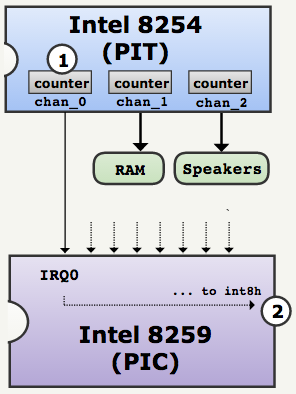
\includegraphics[width=.5\textwidth]{imgs/drawings/heatbeats.pdf}
 \end{figure}
\par
frequency = 1193181 / (value * 60)\\
Inverse Frequency Sound format\\
\par
\begin{figure}[H]
\centering
 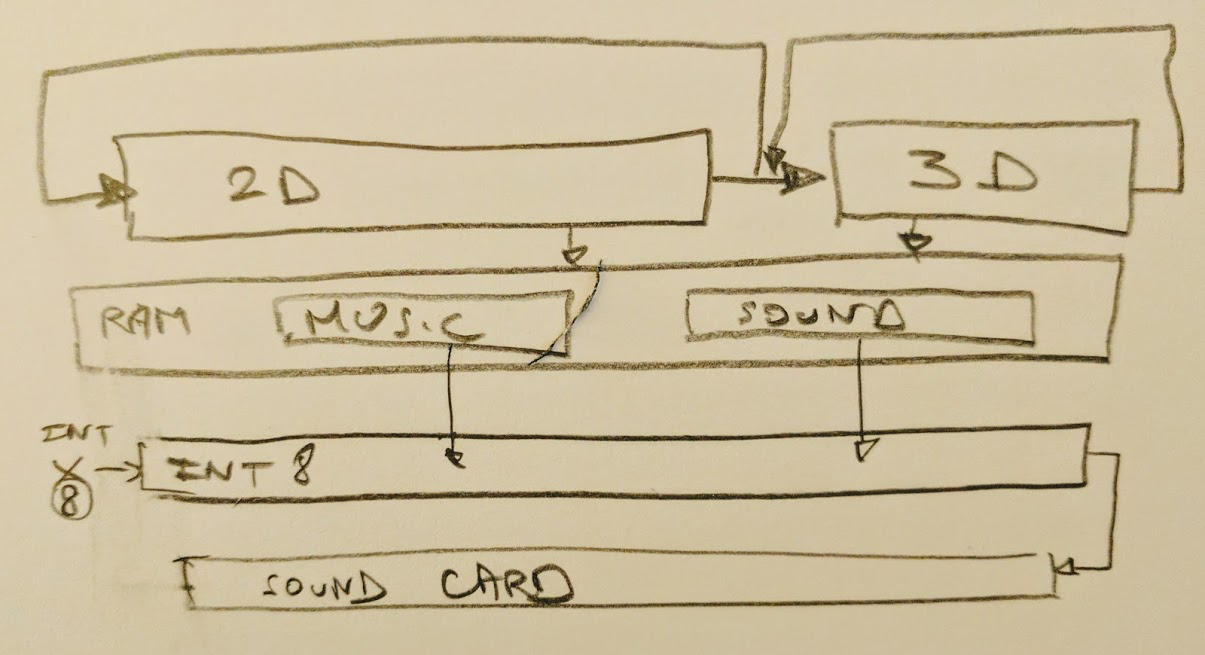
\includegraphics[width=\textwidth]{imgs/drawings/three_blocks.png}
 \end{figure}

Different things could happen depending on the hardware available:
\begin{itemize}
\item With the default PC speaker or with , the isr is set on slow: 140Hz
\item With an adlib or Disney Sound source, the isr is set on fast: 700Hz
\item With Sound Blaster, the isr is set on extreme: 7000Hz
\end{itemize}
Every time the ISR triggers, it takes care of feeding music and audio to the sound chip and also updates TimeCount variable, the heat of the whole system, at 70Hz (like VGA refresh rate).\\
\par
Because the engine uses triple buffering, it is completely decoupled from the VGA refresg rate (70Hz). Yet it needs something not only to pace itself (not render too fast) and to keep track of wall time (so the player is presented with a linear game time progression). This is where the sound system performs two tasks. Not only the XXX chips triggers at a regular interval, it also updates a global variable (\cw{TimeCount}) at 70Hz. This variable is used in the renderer to make sure at least 1/70th of a second has passed before rendering something again but also to pace actor thinking (so player movement is proportionnal to frame rate and actor also think proportionnaly).\\
\cw{CalcTics} maintains \cw{ticks} variable: The amount of walltime since last frame. An action takes a certain number of ticks.\\
\par
It works but there is a major flaw with this technique: The engine is non-deterministic. Recording and replaying a demo, even on the same machine cannot work.\\\par
haha joke about LONG time.\\
\bu{Trivia :} When playing a recording, the engine bypasses the timer and hardcoded tics: (tics = DEMOTICS;). The demo was likely recorded at 15fps which is consistent with what a 386DX33 would have produced

haha: // if the game was paused a LONG time
VGA: 70Hz
audio: Depends on quality, three levels of fidelity.

\par
Stereo system:\\
\par
The sound source is rotated with the same formula as the raycaster. Using SOH-CAH-TOA. Intensity is hardcoded 0-15:\\
\par
\begin{figure}[H]
\centering
 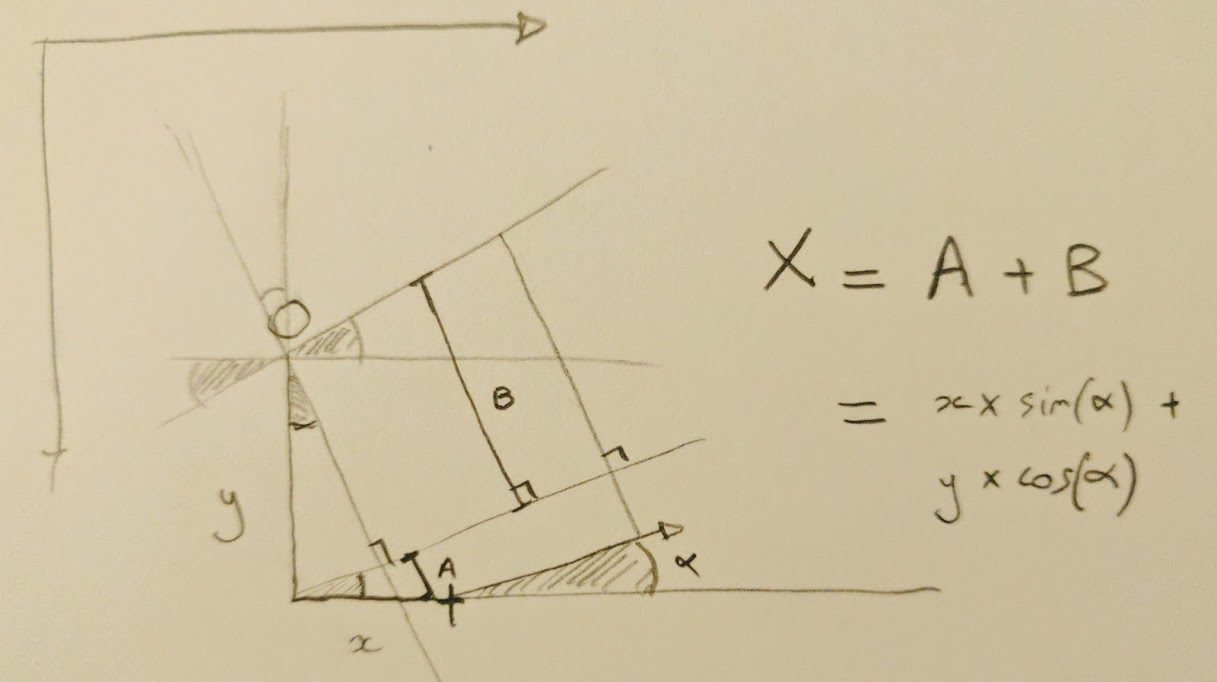
\includegraphics[width=\textwidth]{imgs/drawings/audio_y_rotate.png}
 \end{figure}
 \par
 \begin{figure}[H]
\centering
 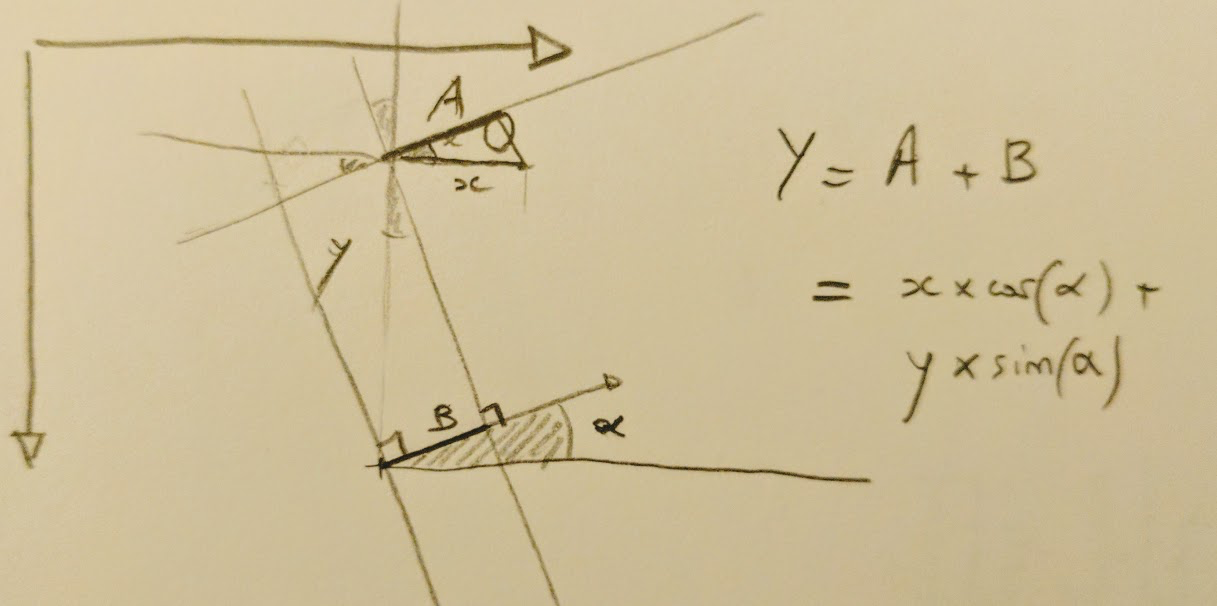
\includegraphics[width=\textwidth]{imgs/drawings/audio_x_rotate.png}
 \end{figure}
\par
In sound part, trivia with a bunch of translations: https://www.gamefaqs.com/pc/564603-wolfenstein-3d/faqs/1824\\
Talk about morse code in episode 3 and 6, echo with romero head in doom2\\
"BLASTER" oldschool parsing.
\section{Pseudo random generator}
US\_RndT\\
rndtable\\
During dying randon generation is done differently.








